\documentclass[a4paper,12pt]{article}

\usepackage{amsmath}
\usepackage{graphicx}
\usepackage{subcaption}

\author{Thorvald Ballestad}
\title{Interacting particles in 2D sphere\\Numerical assignment statistical physics}

\begin{document}
\maketitle

\section{Introduction}
This document is not intended as a formal report.
It is an informal presentation of the results of the project.

\section{Theory}
From the equipartition theorem:
\begin{equation}
  k_B T = E[\frac12 v^2].
\end{equation}\\

The Boltzmann distribution:
\begin{equation}
  P(v_x) = \sqrt{\frac{m}{2\pi k_B T}} e^{-\frac{v_x^2}{2 k_B T}}.
\end{equation}

Using inital conditions where the velocities is normalized such that
$$
\frac{1}{2N} \sum v^2 = 1,
$$
one gets that $k_B T = 1$, and consequently
$$
P(v_x) = \frac{1}{2\pi} e^{-\frac12 v_x^2}.
$$\\

The force on the particles on the wall, is given by the gradient of the potential,
$$
F_w = \sum K(r_i - R) \Theta(r_i - R).
$$
Using the definition of pressure, one get the pressure
$$
P = \frac{F_w}{2\pi R}.
$$

By the ideal gas law (in 2D), one has
$$
\frac{p A}{N} = k_B T = 1,
$$
which should of course hold also for $E[p]$.

\section{Method}
The method will not be discussed in depth here, as it is based on the given code.
A few aspects heed mentioning, however.
The simulation is written in Julia, and the code is delivered together with this document.
The code base is distributed on several files.
The main code lays in \verb|utlis.jl|.
The other files are ment to solve the different problems of the excercise, and call function from \verb|utils.jl|.
The main difference in the datastructure, as compared to the given code, is that positions and velocities are stored as complex numbers.
This is to leverage the built in support for complex numbers, with all the helper functions and specialized routines this offers.
In the author's opinion, this greatly improves the readability of the code.

\section{Results and discussion}
\subsection{Single particle}
Firstly, it is of importance to find a suitable time step, that provides sufficient precision.
Figure \ref{fig:error_one} shows relative error in energy with different values for dt.
The simulation was run with $K = 5$.
$dt = 0.1$ performs reasonably well, with relative error no more than 0.01.
Using this time step, we simulate figure \ref{fig:traj_one}.
Notice that the particle cannot reach the positions close to the origin, it is locked in an outer band.
Thus, this model is not ergodic, and statistical mechanics theory does not apply.
\begin{figure}[ht]
  \centering
  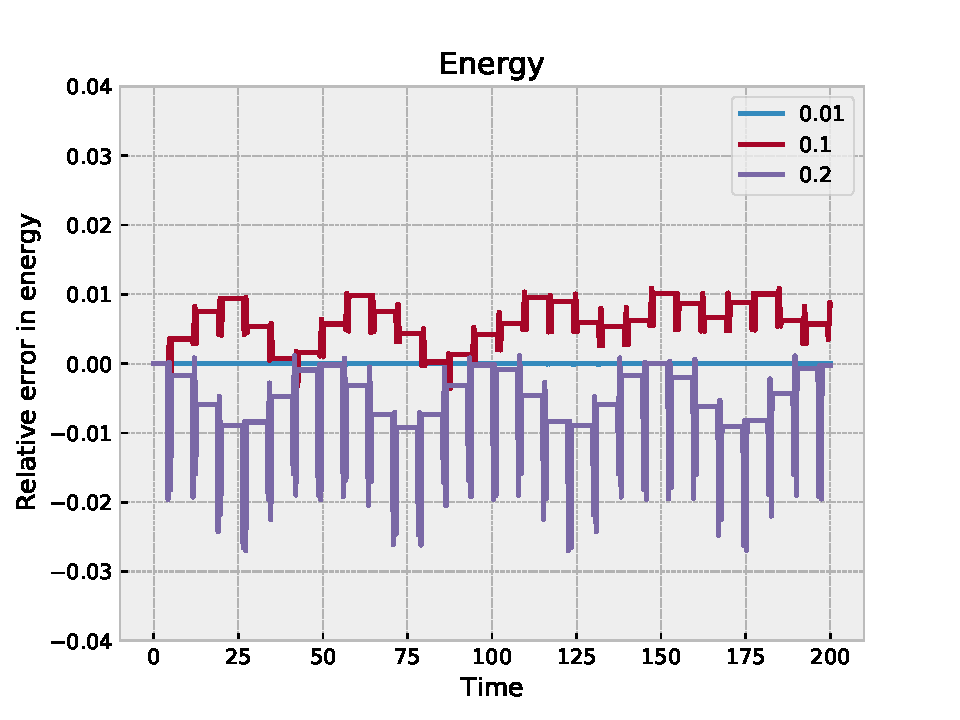
\includegraphics[width=0.75\textwidth]{media/errors_one_particle}
  \caption{Relative errors for different dt with one particle. Wall hardness parameter $K=5$.\label{fig:error_one}}
\end{figure}

\begin{figure}[ht]
  \centering
  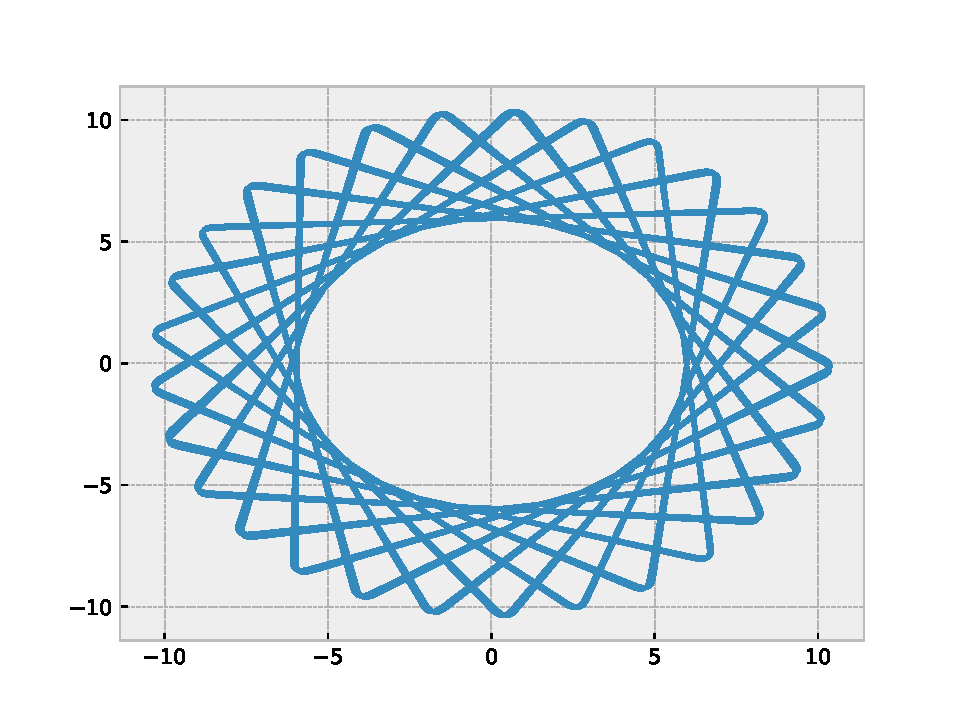
\includegraphics[width=0.75\textwidth]{media/trajectory_one_particle}
  \caption{Trajectory of a single particle, to $T=1000$\label{fig:traj_one}}
\end{figure}



\subsection{Multiple particles}
Extending the simulation to multiple particle, the results become quite different.
As seen in figure \ref{fig:traj_two}, \ref{fig:traj_three}, and \ref{fig:traj_five}, showing the trajectories of two, three, and five particles respectively, the particles are no longer ``locked'' in a fixed band.
The center positions are also visited.
In figure \ref{fig:traj_multiple} the density plot of ten particles is shown.
The distribution is fairly uniform.

\begin{figure}[hp]
  \centering
  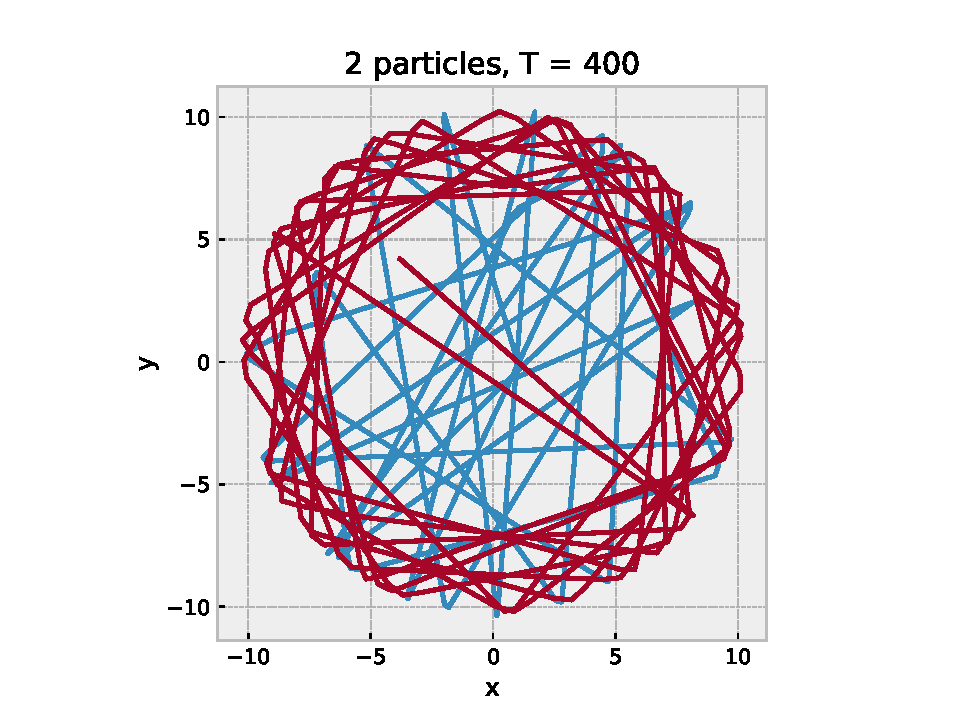
\includegraphics[width=.75\textwidth]{media/trajectory_two_particles}
  \caption{Trajectories of two particle, to $T=700$\label{fig:traj_two}}
\end{figure}

\begin{figure}[hp]
  \centering
  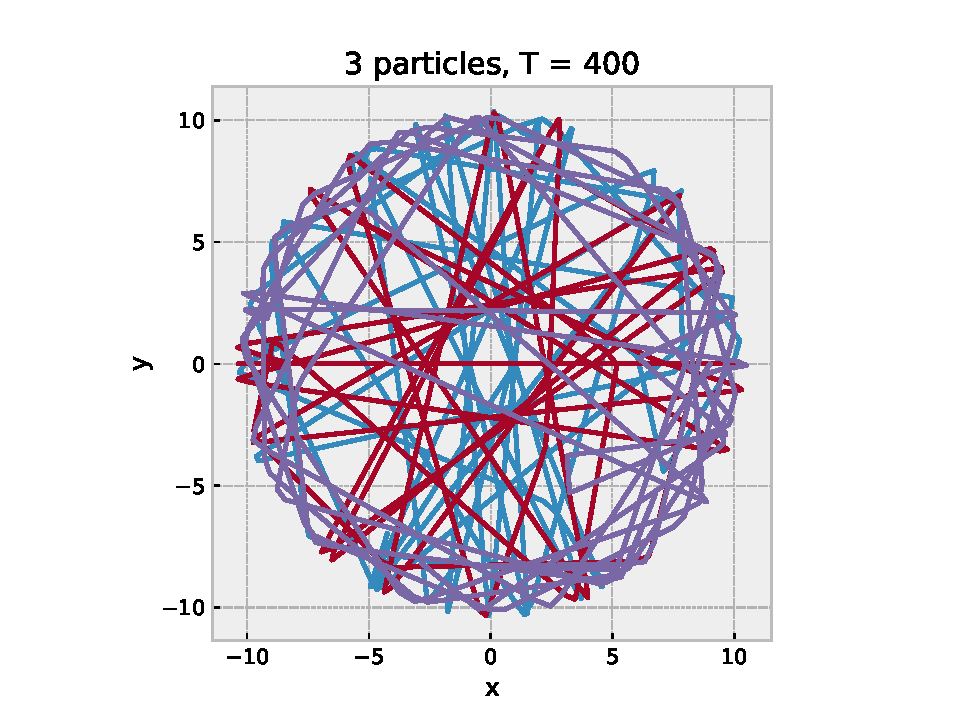
\includegraphics[width=.75\textwidth]{media/trajectory_three_particles}
  \caption{Trajectories of three particle, to $T=700$\label{fig:traj_three}}
\end{figure}

\begin{figure}[hp]
  \centering
  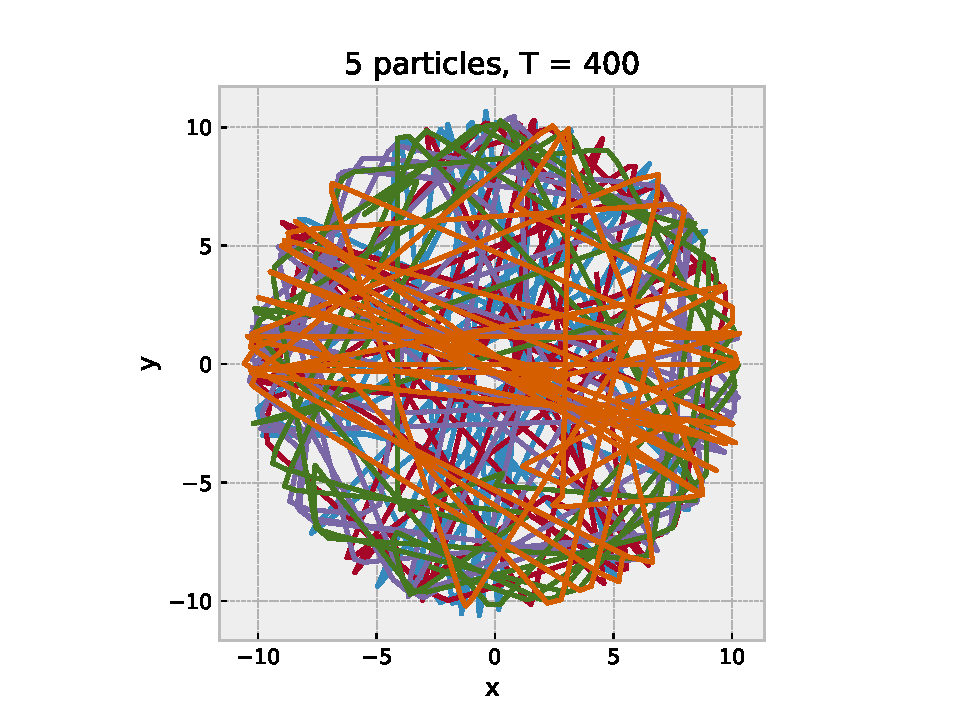
\includegraphics[width=.75\textwidth]{media/trajectory_five_particles}
  \caption{Trajectories of five particle, to $T=700$\label{fig:traj_five}}
\end{figure}

\begin{figure}[htp]
  \centering
  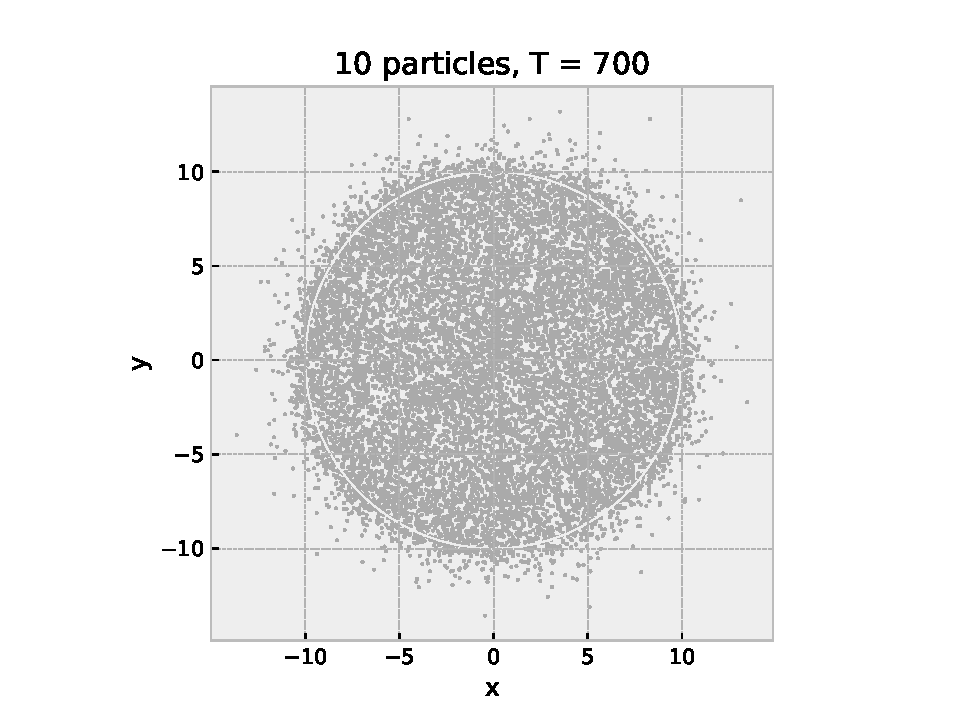
\includegraphics[width=.75\textwidth]{media/trajectory_ten_particles}
  \caption{Density plot for ten particles, to $T=700$\label{fig:traj_multiple}}
\end{figure}


Statistical mechanics theory says that the inital condition should not matter; the statistical results are not affected by inital state.
A naive first approximation to testing if this model captures this requirement, is to simulate a system where the energy is distributed non-uniformly.
Fiugre \ref{fig:energy_dispersion} shows a simulation with three particles, where in the inital state, only one particle has velocity different from zero -- the other two starts at rest.
However, through the simulation, the energy distribution flucutates.
This is in correspondence with statistical mechancis theory, it appears that the systems tends towards visiting all possible states.

\begin{figure}[htp]
  \centering
  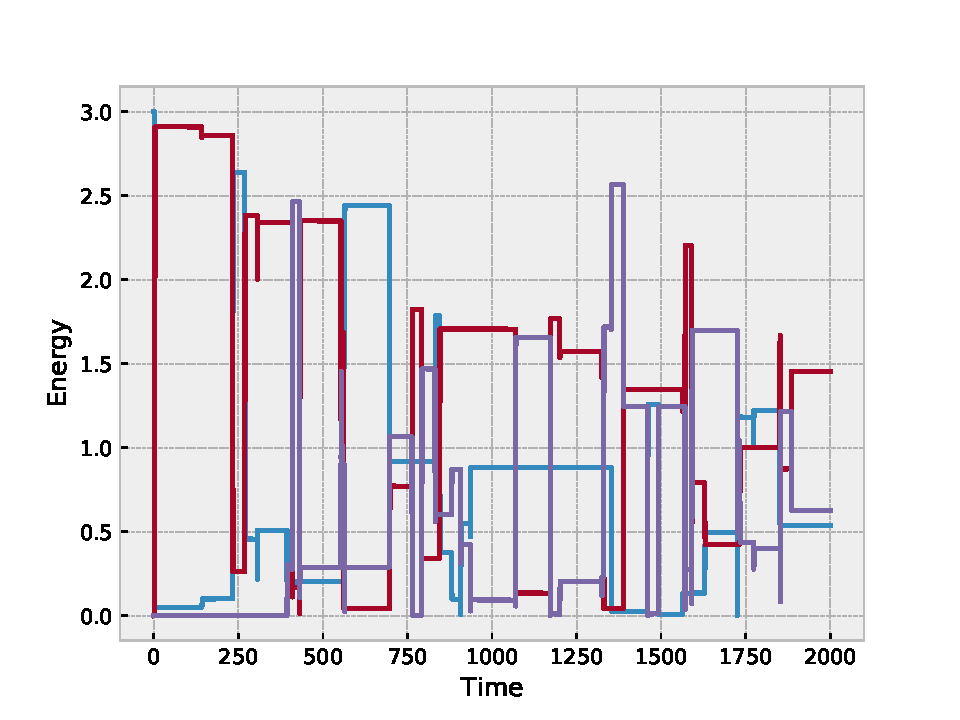
\includegraphics[width=.75\textwidth]{media/energy_dispersion}
  \caption{Distribution of energy among three particles as a function of time. Notice that initally, only one particel has energy, the others are at rest.\label{fig:energy_dispersion}}
\end{figure}


Considering one particle in the simulation, we can apply theory from the canonical ensable.
Here, one expect the distribution to follow the Boltzmann distribution, which is given in the theory section.

The velocity distribution form simulating 10 particles until $T=600$ is shown in figure \ref{fig:velocity_distribution}.
It is clear that the simulated distribution follows the distribution from the canonical theory.
$k_B T = \frac12 E[v^2]$ was in the simulatin found to be 1.028, which is close to the correct value of 1.

\begin{figure}[htp]
  \centering
  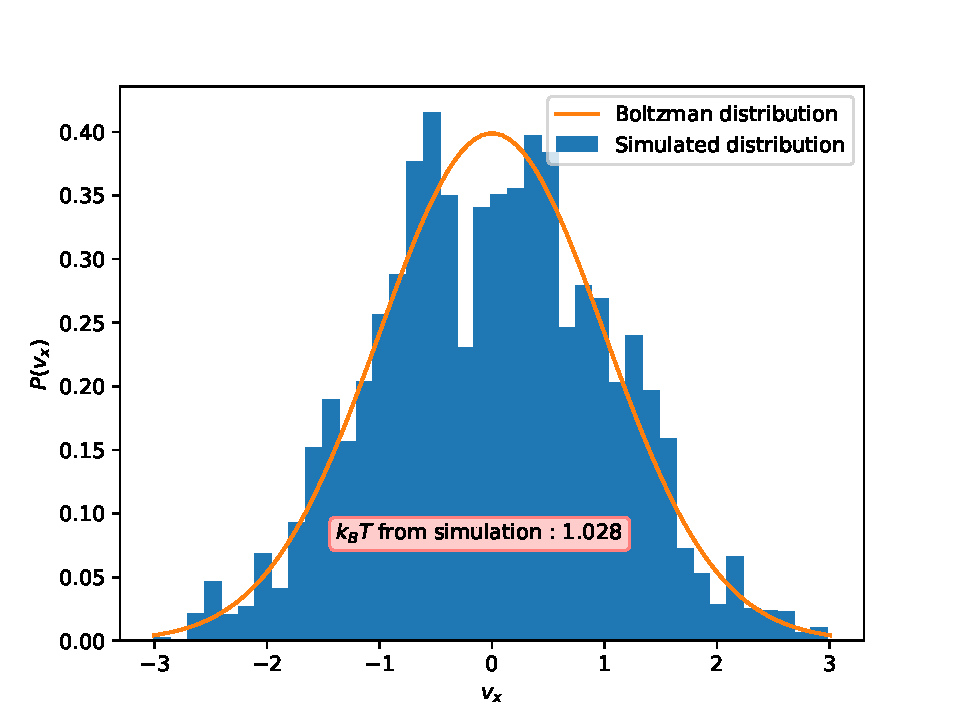
\includegraphics[width=.75\textwidth]{media/velocity_distribution}
  \caption{Velocity distribution for simulation of 10 particles until $T=600$.\label{fig:velocity_distribution}}
\end{figure}

In figure \ref{fig:pressures} the pressure on the box as a function of time is shown.
Following the ideal gas law, the value of $\frac{p A}{N}$ should be constant and equal to $k_B T$.
In the simulation, using the expectation value of the pressure for $p$, this value was fairly close to the correct value, 1, in each case.
The simulation results are shown in table \ref{tab:pressures}.

\begin{table}[h!]
  \centering
  \begin{tabular}{lll}
    N& R& $\frac{E[p] A}{N}$\\
    \hline
    5& 6& 0.930\\
    10& 10& 1.000\\
    15& 13& 1.044\\
    5& 10& 1.080
  \end{tabular}
  \caption{Values of $\frac{E[p] A}{N}$ for various $N$ and $R$.\label{tab:pressures}}
\end{table}

\begin{figure}[htp]
  \centering
  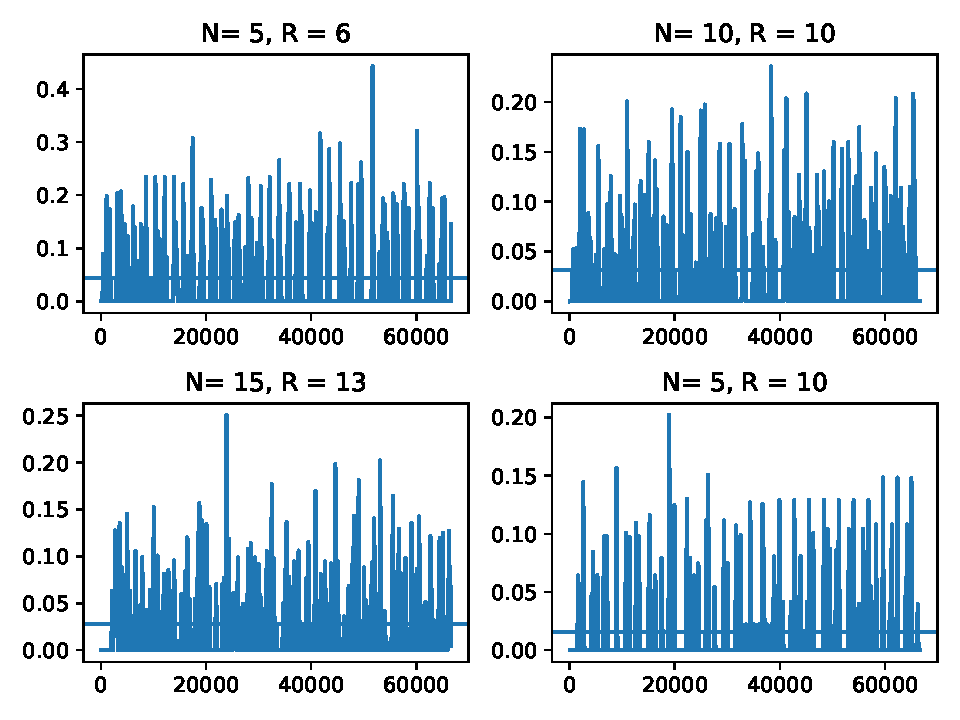
\includegraphics[width=.75\textwidth]{media/pressures}
  \caption{Pressure as a function of time for different number of particles and radii.
    The value of $E[P] A /N$ was found to be 0.930, 1.000, 1.044, and 1.080.
    The horizontal lines represents the theoretical values.
    \label{fig:pressures}}
\end{figure}

\section{Conlusion}
This model captures many important results and behaviours from statistical mechanics.

\end{document}
